
\subsection{First order equaitons for mono disperse fore after axisymmetric particle suspension}

To highlight the importance of the first order moments equations, we first take the example of mono-disperse solid axis symmetric particle suspension. 
In this case it is known that the orientation of the particles play a key role in the drag and hydrodynamic first moment models.
It is therefore primordial to fix a first order system of equation to capture this phenomenon.  
\begin{figure}[h!]
    \centering
    \hfill
    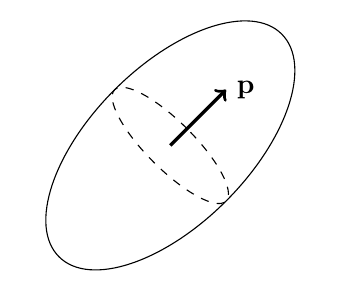
\begin{tikzpicture}[rotate=45]
        \draw(0,0) ellipse (2 cm and 1 cm);
        \draw[dashed](0,0) ellipse (0.3 cm and 1 cm);
        \draw[->,very thick](0,0) --++ (1,0)node[right]{$\textbf{p}$};
    \end{tikzpicture}
    \hfill
    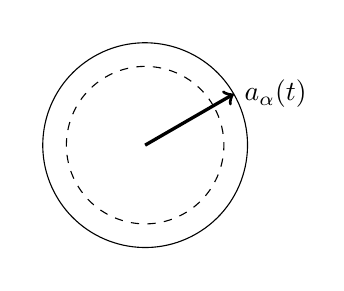
\begin{tikzpicture}[rotate=30]
        \draw(0,0) ellipse (1.3 cm and 1.3 cm);
        \draw[dashed](0,0) ellipse (1 cm and 1 cm);
        \draw[->,very thick](0,0) --++ (1.3,0)node[right]{$a_\alpha(t)$};
    \end{tikzpicture}
    \hfill
    \caption{Scheme of an axis symmetric particle with fore after symmetry and orientation normal vector \textbf{p}.}
    \label{fig:scheme2}
\end{figure}

\subsubsection*{Closures}
Initially we aim to solve the momentum equation for the fluid and particle phase \ref{eq:hybrid_avg_dt_rhou} and \ref{eq:hybrid_avg_dt_dp_alpha}. 
As previously mentioned these equations contain the following closures terms : $\oneavg{\textbf{T}}, \pnnavg{\textbf{f}_\alpha}, \pnnavg{\textbf{t}_\alpha}$ and $\pnnavg{\textbf{S}_\alpha}$ if we discard the fluctuation terms.
The closure for the averaged stress tensor appearing in \ref{eq:hybrid_avg_dt_rhou} can be express assuming solid unreformable motion inside the particles, with, \citep{jackson1997locally},
\begin{equation*}
    \phi_1\oneavg{\textbf{T}}
    =  - \phi_1\oneavg{p}\textbf{I}
    + \mu_1 \avg{\textbf{E}}
\end{equation*}
where $p$ is the pressure conditionally averaged on the phase $1$ and $\avg{\textbf{E}} = \nablab \avg{\textbf{u}} + (\nablab \avg{\textbf{u}})^T$ is the mean rate of strain tensor. 
Notice that the bulk velocity appearing in the above expression is in fact, $\avg{\textbf{u}} = \phi_1\oneavg{u} + \pnavg{\textbf{u}_\alpha} + \nablab\cdot (\pnavg{\mathcal{P}_\alpha})$.
Thus, the moment of momentum appear explicitly in the closure of the stress. 
Regarding the drag force, in  \citet{brenner1963resistance} they demonstrate that in low but finite inertia for an arbitrary shaped particle it could be expressed as,
\begin{equation}
    \textbf{f}_\alpha = 3 \pi \mu L \left[
        \textbf{R}_\alpha \cdot \textbf{U}
        + \frac{3}{16} Re  \left(
            3 \textbf{R}_\alpha 
            - \textbf{I} (\textbf{R}_\alpha : \textbf{e} \textbf{e})
        \right)
        \textbf{R}_\alpha\cdot  \textbf{U}
    \right]
\end{equation}
where $\textbf{U} = \oneavg{\textbf{u}}(\textbf{x}_\alpha)  - \textbf{u}_\alpha$ , $\textbf{e} = \textbf{U}/|\textbf{U}|$. 
and,  $\textbf{R}_\alpha$ is the resistance tensor in the laboratory frame. 
Besides, for axisymmetric particles with orientation vector \textbf{p} (sse \ref{fig:scheme2}) it can be shown that $\textbf{R}_\alpha = (R_{||} - R_\bot) \textbf{pp} + R_\bot \textbf{I}$, where $R_{||}$, $R_\bot$ are scalar coefficients \citep{guazzelli2011,kim2013microhydrodynamics}. 
Regarding the hydrodynamic torque applied on an asymmetric particle it can be expressed in Stokes regime as, 
\begin{equation}
    \textbf{t}_\alpha 
    = 
    \textbf{R}_{\omega T}\cdot \mathbf{\Omega}
     + \textbf{R}_{TU} \cdot \textbf{U} 
\end{equation}
where the first term represent the torque acting on the particle due to its translation,
with $R_T$ a correlation also function of the shape and $\textbf{U}$.
It must be noted that this relation remain partially true in low but finite inertial regime. 
Note that the correlation,  $R_T, R_{||} , R_{\bot}$ can be found in \citet{fintzi2023inertial} for cylindrical particles in dilute regime. 
And the second term represent the torque due to its rotation vector $\omega_\alpha$, where $\textbf{R}_{\omega T}$ is the resistance tensor linking rotation and torque \citet{pierson2021hydrodynamic} for inertial regime.  
Both $\textbf{R}_{\omega T}$ and $\textbf{R}_{TU}$ terms are function of the orientation of the particle \textbf{p}.
Closure for $\textbf{S}_\alpha$ can also be found but in the stokes regime only, 
indeed theoretical results are given in \citet[p 62]{kim2013microhydrodynamics}. Nevertheless, we do not provide them here as the expression is rather complicated. 
From the view of these closure terms we can see that in addition to the zeroth order terms, it is primordial to determine quantitatively the tensor $\textbf{pp}$, the rate of rotation $\omega_\alpha$ and the moment of momentum $\mathcal{P}_\alpha$. 

\subsubsection*{Dipole equations}
Let consider a solid axis symmetric particle with fore after symmetric such that exposed in \ref{fig:scheme2}. 
Due to axis symmetric nature of the particle we can stipulate that, 
\begin{equation}
    \mathcal{V}_\alpha =  \textbf{pp} (V_\alpha^{||} - V_\alpha^\bot) 
    +  \textbf{I} V_\alpha^\bot
    \label{eq:V_definition}
\end{equation}
with $V_\alpha^{||}$, $V_\alpha^\bot$ being constant values related to the volume and shape of the particle. 
Besides, the velocity fields in inside each particle's domain can be deduced from solid body assumption, $\textbf{u}_2(\textbf{x}_\alpha + \textbf{r},t) = \textbf{u}_\alpha + \omega_\alpha \times \textbf{r}$ where $\omega_\alpha$ is the rotation vector of the particle $\alpha$.
By making use of this velocity decomposition it is easy to show that,
\begin{align}
    \mathcal{P}_\alpha/\rho_2
    &=  \omega_\alpha \times \left[
        \textbf{pp}(V_\alpha^{||} - V_\alpha^\bot) 
        + \textbf{I} V_\alpha^\bot
    \right]
    \label{eq:P_edfinition}\\
    2\mathcal{S}_\alpha/\rho_2
    &=  (V_\alpha^{||} - V_\alpha^\bot) \left(
        \omega_\alpha \times
        \textbf{pp}
        + \textbf{pp} \times \omega_\alpha
    \right)
    \label{eq:S_definition}\\
    \mu_\alpha / \rho_2
    &= \omega_\alpha \cdot \left[
        \textbf{pp} 
    (V_\alpha^{||}  - V_\alpha^{\bot} ) 
    - \textbf{I}(V_\alpha^{||} + V_\alpha^{\bot})
    \right]
    = \omega_\alpha \cdot\mathcal{I}_\alpha
    \label{eq:mu_definition}
\end{align}
Remark that  using the definition of $\mathcal{I}_\alpha$ yields a much simpler expression for $\mu_\alpha$. 

It is then trivial to show that from \ref{eq:hybrid_avg_dt_dV_alpha},\ref{eq:S_definition} and \ref{eq:V_definition} we obtain the second order moment of volume conservation,
\begin{multline}
    \pddt (\pnavg{\textbf{pp}})
    + \nablab \cdot (
        \pnavg{\textbf{pp}}\pnnavg{\textbf{u}_\alpha}
        + \pnavg{\textbf{pp}'\textbf{u}_\alpha'}
        )
    = 
    \pnavg{\textbf{pp}} \times \pnnavg{\omega_\alpha}\\
    + \pnnavg{\omega_\alpha} \times \pnavg{\textbf{pp}} 
    + \pnavg{\textbf{pp}' \times \omega_\alpha'}
    +\pnavg{\omega_\alpha' \times \textbf{pp}'}
    \label{eq:hybrid_avg_dt_pp}
\end{multline}
In agreement with \citet{advani1987use} which found similar results except that they brought empirical expression for the fluctuation terms. 
Also, notice that the RHS of the equation is in fact the expression of $\pnnavg{\mathcal{S}_\alpha} /{ \rho_2 (V_\alpha^{||} - V_\alpha^\bot)}$.

An equation for the rotation rate $\pnnavg{\omega_\alpha}$ can be obtained by, manipulating the angular momentum balance  \ref{eq:hybrid_avg_dt_dmu_alpha}, and using \ref{eq:mu_definition} and \ref{eq:hybrid_avg_dt_pp}, which gives,
\begin{multline}
    \left(
        \pnnavg{\textbf{pp}} 
        - \textbf{I}\frac{V_\alpha^{||} + V_\alpha^\bot}{V_\alpha^{||} - V_\alpha^\bot}
    \right)\left[
        \pddt (\pnavg{\omega_\alpha})
        + \nablab \cdot (
            \pnavg{\omega_\alpha}\pnnavg{\textbf{u}_\alpha}
            + \pnavg{\omega_\alpha'\textbf{u}_\alpha'})
        \right]\\
    +  \pnavg{\omega_\alpha}
    \cdot(\pnnavg{\omega_\alpha} 
    \times \pnnavg{\textbf{pp}})
    = \frac{\pnavg{\textbf{t}_\alpha}}{\rho_2}
    -\pnavg{\omega_\alpha' \cdot (\omega_\alpha \times \textbf{pp})'}
    +\pnavg{\omega_\alpha' \times \textbf{pp}}
    - \pnavg{\textbf{pp}'\dot{ \omega_\alpha}'}
\end{multline}
On the RHS we can observe that there is numerous closure fluctuation terms.  
\tb{FIND ref of this equations}
\subsubsection*{Stress equation}

Lastly, once we solved for $\pnnavg{\textbf{pp}}$ and $\pnavg{\omega_\alpha}$ we can deduce $\mathcal{S}_\alpha$ thanks to \ref{eq:S_definition}.
Afterward, we compute the integral of the undefined internal stress with \ref{eq:hybrid_avg_dt_dS_alpha}, which yield in our case, 
\begin{multline}
    \pnavg{\int_{\Omega_\alpha} 
        \mathbf{T}_2
    d\Omega}
    =  
      \frac{1}{2}\frac{\pnavg{\textbf{S}_\alpha}}{\rho_2}
    - \pddt \pnavg{\mathcal{S}_\alpha}
    - \nablab\cdot(\pnavg{\mathcal{S}_\alpha \textbf{u}_\alpha})\\
    - (V_\alpha^{||} - V_\alpha^\bot) \pnavg{
        (\omega_\alpha \times \textbf{p}) (\omega_\alpha \times \textbf{p}) } 
    -V_\alpha^\bot \pnavg{\textbf{I} \omega_\alpha^2 -\omega_\alpha\omega_\alpha }
    \label{eq:T2_definition}
\end{multline}
Then considering the particle nature it is possible to deduce its mean deformation from the stress integral, and validate or not the irreformability hypothesis made at start. 
It is also possible to compute the trace of the stress using \ref{eq:hybrid_avg_dt_dD_alpha}, yielding in this case, 
\begin{equation}
    \pnnavg{\int_{\Omega_\alpha} 
        \textbf{I}:\mathbf{T}_2
    d\Omega}
    =  
     (V_\alpha^{||} + V_\alpha^\bot) \pnnavg{
    \omega_\alpha^2} 
    - (V_\alpha^{||} - V_\alpha^\bot) \pnnavg{
    \omega_\alpha\omega_\alpha :  \textbf{pp}}
    + \pnnavg{\textbf{M}_\alpha} : \textbf{I}
\end{equation}
where we considered that the volume of the particle remained constant. 
This equation means that the rotational acceleration contribute to the isotropic particle pressure. 


In a pure rigorous manner the equivalent bulk stress of the suspension yield, 
\begin{equation*}
    \avg{\textbf{T}} = 
    \phi_1 \oneavg{\textbf{T}} 
    + \pnavg{\int_{\Omega_\alpha} \mathbf{T}_2 d\Omega}
    -\nablab\cdot \pnavg{\int_{\Omega_\alpha} \textbf{r}\mathbf{T}_2 d\Omega}
    + \ldots
\end{equation*}
Where the first and second terms on the RHS are given by \ref{eq:T_definition} and \ref{eq:T2_definition}, and the last one can be obtained with the third order moment of momentum equations. 
Anyhow if we neglect this last term and if the solid motion hypothesis remain true we can determine the bulk stress with the relation :
\begin{multline*}
    \avg{\textbf{T}} = 
    - \phi_1\oneavg{p}\textbf{I} 
    + \mu_1(\nablab \avg{\textbf{u}} + (\nablab \avg{\textbf{u}})^T) 
    + \frac{1}{2}\frac{\pnavg{\textbf{S}_\alpha}}{\rho_2}
    - \pnavg{\ddt \mathcal{S}_\alpha}\\
    - (V_\alpha^{||} - V_\alpha^\bot) \pnavg{
        (\omega_\alpha \times \textbf{p}) (\omega_\alpha \times \textbf{p}) } 
    -V_\alpha^\bot \pnavg{\textbf{I} \omega_\alpha^2 -\omega_\alpha\omega_\alpha }
\end{multline*}

\section{Compressible air bubble}
\begin{itemize}
    \item Conisder compressible air bubble such as (88) in \citet{zhang1994ensemble}
    \item From \ref{eq:hybrid_avg_dt_dD_alpha} derive the \textit{Rayleigh-Plesset} equation Similarly to (88) of Zhang. 
    \item Do the same calculation than Lhuiller's note but for compressible bubble instead of mass transfer equations section 4.2 de ses notes
\end{itemize}
\section{Bulk stress in drop with linear internal motion}

\begin{itemize}
    \item compute the bulk stress with \ref{eq:T2_definition}
\end{itemize}


